%%%%%%%%%%%%%%%%%%%%%%%%%%%%%%%%%%%%%%%%%%%%%%%%%%%%%%%%%%%%%%%%%%%%%%%%%%%%%%%%
%   Chapter 3
%%%%%%%%%%%%%%%%%%%%%%%%%%%%%%%%%%%%%%%%%%%%%%%%%%%%%%%%%%%%%%%%%%%%%%%%%%%%%%%%
\chapter{Experimentation} \label{chap:exper}

%%%%%%%%%%%%%%%%%%%%%%%%
% Hardware Setup Section
\section{Hardware Setup} \label{sec:hardware}

All experimental data was taken using Novatel Propak v3 GPS receivers with pinwheel antennas, identical to those used in \cite{scottthesis}. All positioning computation was conducted on an Apple MacBook Pro Laptop running Ubuntu Linux 12.04.1 in a Parallels virtual machine which was located in the rearmost vehicle. This machine also hosted and displayed the GUI during all test runs. Novatel data was relayed directly from the receiver placed in the lead vehicle to the positioning computer through the use of two XTend-PKG $900~MHz$ radio modems operating at a power output of $1~W$ and connected via RS232-USB adapters. This eliminated the need for an additional computer, which was found to introduce unacceptable latency into the system. In this manner, a single central hub was able to host the MOOS database while controlling all receivers and data flow to all position algorithms without the needing two-way radio communication for the GUI. The complete hardware package placed inside the lead vehicle is shown in Fig. \ref{fig:hardwarelead}, including power connections and externally mounted antennas. Fig. \ref{fig:hardwarefoll} depicts the hardware placed in the following vehicle, which includes the same components placed in the lead vehicle, but serve a different purpose, as shown in Fig. \ref{fig:hardwareflow}

\begin{figure}[ht] \centering
    \begin{minipage}[b]{0.45\linewidth} \centering 
        \includegraphics[width=\textwidth]{./figs/driver_view.jpg}
        \caption{GUI as presented to the driver} \label{fig:driverview}
    \end{minipage}
    \hspace{0.5cm}
    \begin{minipage}[b]{0.45\linewidth} \centering
        \includegraphics[width=\textwidth]{./figs/foll_hardware.jpg}
        \caption{Follower interior hardware} \label{fig:hardwarefoll}
    \end{minipage}
\end{figure}

% data collection
The stream of available data may be divided into two categories: raw GPS measurements used to compute a relative path online, and the measurements coming either the receiver or DAF algorithm which is displayed on-screen. When conducting experimental trials for formal analysis, the latter is recorded in order to capture exactly what was displayed to the following driver and examine their performance. The former is excluded in order to reduce the volume of data throughput and increase computing efficiency, as following distance and lateral path deviation are derived from the relative path and follower velocity alone. However, during the develop-test-refine cycle, the inverse is true; raw GPS measurements alone are recorded (again, neglecting other data for efficiency). This is then replayed to simulate online operation as algorithms are tuned.

\begin{figure}[ht] \centering
    \begin{minipage}[b]{0.45\linewidth} \centering 
        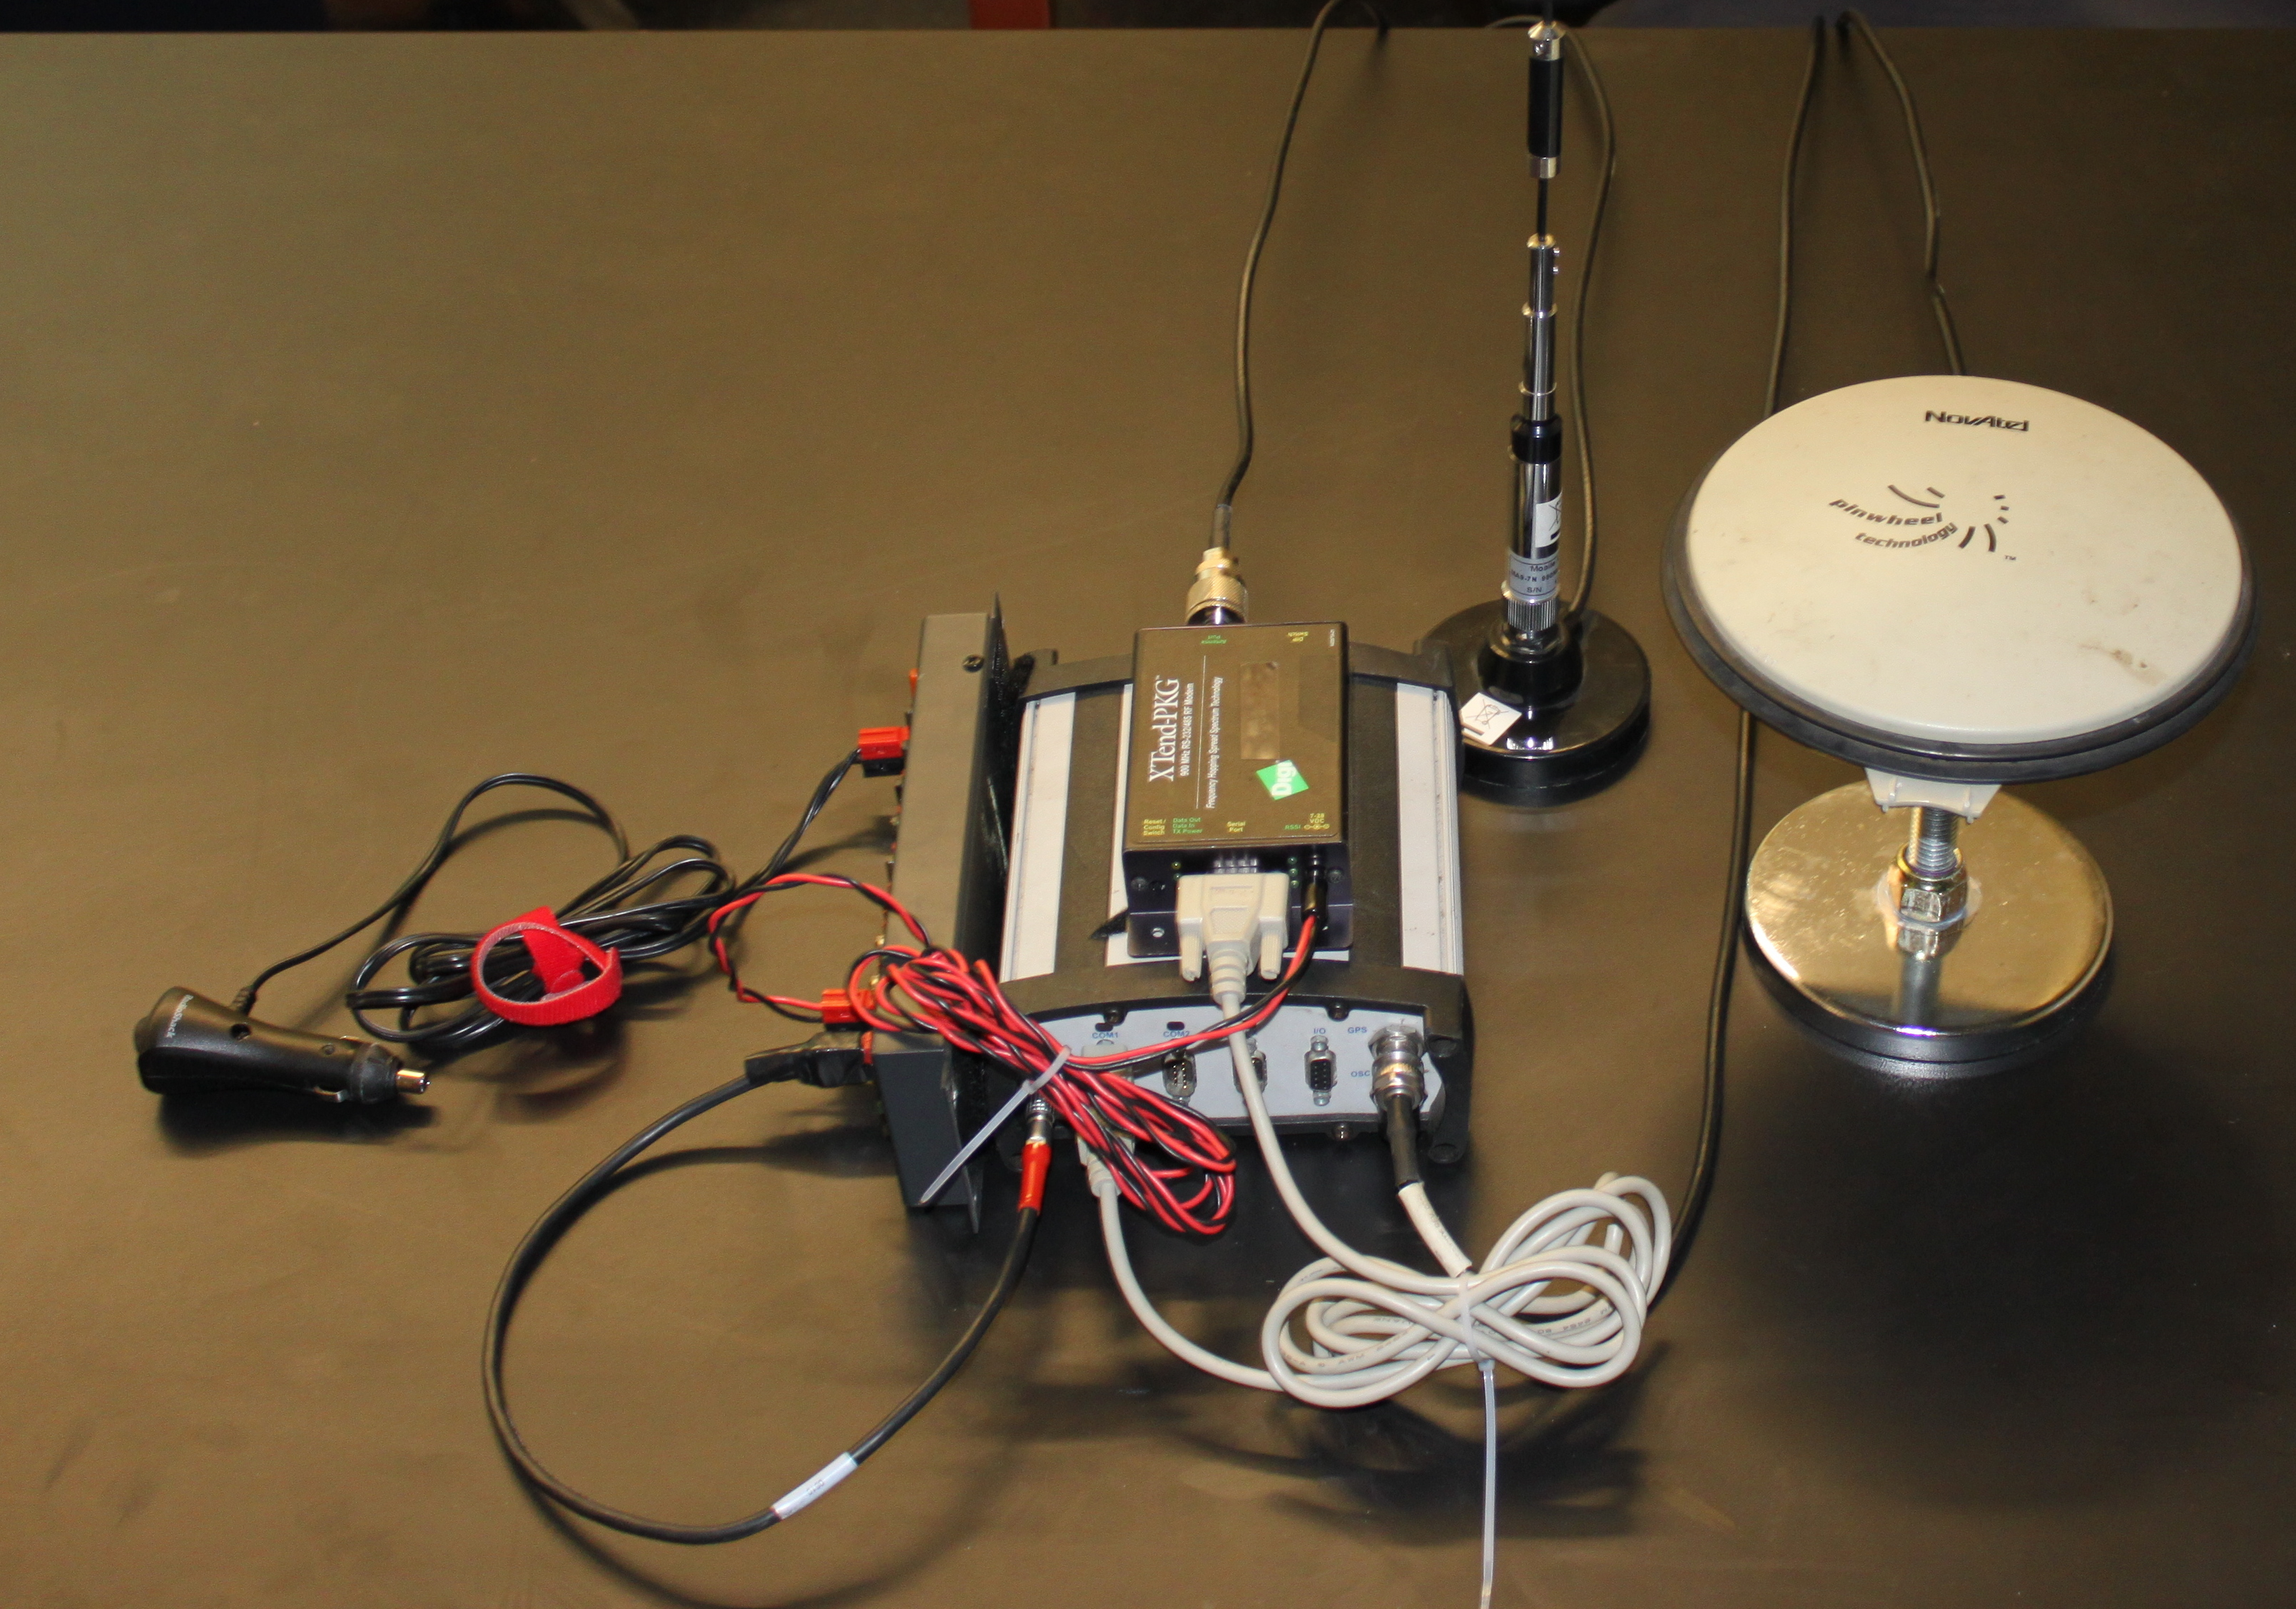
\includegraphics[width=\textwidth]{./figs/lead_hardware.jpg}
        \caption{Equipment used in the leading vehicle} \label{fig:hardwarelead}
    \end{minipage}
    \hspace{0.5cm}
    \begin{minipage}[b]{0.45\linewidth} \centering
        \includegraphics[width=\textwidth]{./figs/foll_antennae.jpg} 
        \caption{Antennaes as placed on either vehicle} \label{fig:antennaefoll}
    \end{minipage}
\end{figure}

%%%%%%%%%%%%%%%%%%%%%%%%%%%
% What tests were performed
\section{Testing} \label{sec:test}
In order to formally quantify the ability of the tools developed in Chap. \ref{chap:gui} to assist convoy drivers in the target circumstances, three tests were devised: a lane change replication test, a target spacing maintenance test, and a limited visibility test. These were also conducted to compare and contrast the two approaches embodied by each GUI. Since the tools developed before are designed for a single leader/follower pair, as few as two vehicles can be used as a convoy.
Until Chap \ref{chap:errprop}, this configuration will be used.

\begin{figure}[ht] \centering
    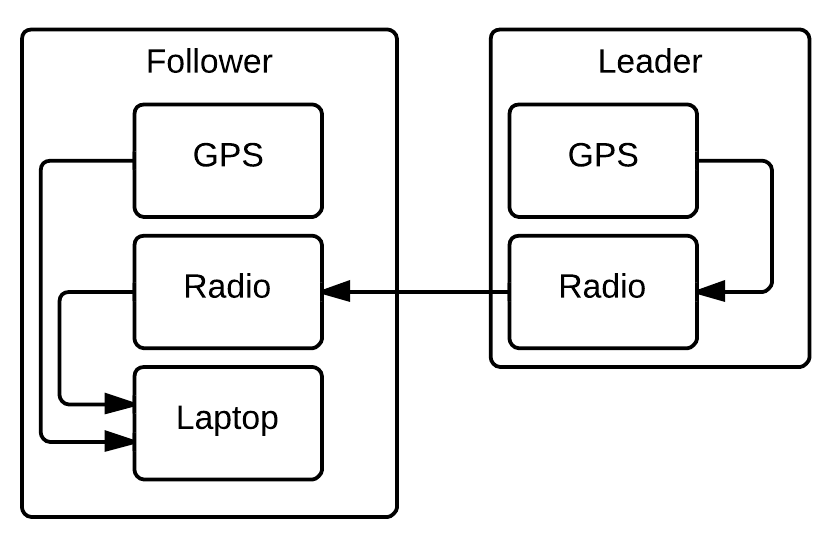
\includegraphics[width=4in]{./figs/hardware_flow.png}
    \caption{Flow of GPS data between leader and follower} \label{fig:hardwareflow}
\end{figure}

%%%% Lane change replication
\subsection{Lane Change Replication Test} \label{sec:lanechangetest}
In determining the usefulness of any tool, it is highly desirable to devise a test which yields concise results that are either completely positive or negative. To this end, a maneuver common in typical roadway driving, the lane change, was used in a situation in which the maneuver could be replicated properly or improperly to produce a binary result. This test takes place on the National Center for Asphalt Technology (NCAT) test track in Opelika, AL, which is a two lane, 1.7 mile oval oval with turns comparable to those found on an interstate highway. The leader rounds a $180^\circ$ turn and upon exiting makes a lane change between any of six cones spaced $10m$ apart along the center stripe at the start of the straightaway. This event is visually obscured from the following driver, who has no foreknowledge of which cone pair will be chosen, so there is a $20\%$ chance of choosing the correct pair simply by guessing. This iteration of this test was performed twice, once with the monolithic GUI and once with the Earth-based GUI. No control run is needed, since a cumulative success rate across all iteration above $20\%$ represents an improvement from driving without navigation assistance. A range of highway driving speeds from 30 mph to 70 mph was used, and forward spacing was not examined except to ensure that it was large enough for the aforementioned visual obstruction.

This focused on aiding a driver in conditions where visibility is totally denied, as foliage and terrain features lie between the two vehicle during the moment of interest. Sensor and display frequencies will play a large role in this outcome. If information is updated with real time interpolation, a delay of at least one timestep (not including calculation time) is present, meaning that a worst-case GPS output frequency of 1.0 Hz will result 1.0 s data lag. For a following vehicle is travelling at 55 mph (24.5872 m/s), a 24.5872 m discrepancy between the path satellite imagery and the actual path. The impact of that behavior is one thing being examined in the lane change replication test. For the monolithic GUI, this test will show whether the range scaling indicators adequately convey distance information so that a driver can determine where to turn, when the interpolation functionality is disabled for rapid updating. The results are outlined in Sec \ref{sec:lanechangetestresults}

%%%% Target Spacing Test
\subsection{Precision Following Test} \label{sec:targetspacingtest}
The lane change replication test one example of implementing the path duplication tool, but does not produce the detailed results necessary for a formal conclusion favoring the usefulness of one GUI over the other. Centimeter-level measurements are available, so it is of great interest to determine whether either tools enables a convoy driver to carry out the following task with this same level of precision. The precision following test begins and ends with both vehicles parked atop the center stripe of the NCAT test track. The lead vehicle accelerates to approximately 45 mph then begins a sinusoidal path with a mean about the center stripe, a period of approximately 10 s, and an amplitude of which puts the wheels of the lead vehicle upon the outermost lane marking at the peaks. Once reaching 45 mph, the magnitude of the leader's ground plane velocity vector will vary according to position on the track. Along the two 180$^\circ$ turns it will be approximately 45 mph, and along the straightaways it will be approximately 65 mph. Throughout the test, the following driver is attempting to maintain a inter-vehicular spacing as low as possible without incurring any distance alerts, and accumulate as little deviation over time as possible. 
This test primarily focused on distinguishing which GUI best provided aid in path duplication; for a comparative analysis, the test was conducted with the aid of each GUI individually, then without any assistance information at all. The results are outlined in Sec. \ref{sec:precisionfollowingresults}

% %%%% Circuit Around NCAT
% \subsection{Varied Driving Test} \label{sec:variedtest}
% The above tests represent very specific scenarii that, while examining situations which commonly arise in convoy driving, did not fully cover the full range of behaviors which are being aided.  A singular test was desired which would at once examine all aspects of the graphical tool and produce broad results over multiple driving scenarii. A route around the NCAT facility was devised which included non-lane driving in environments with plenty of visual references, as well as those without. The skidpad portion of this test is an environment with no visual landmarks by which to localize the leader, as it is a flat, open expanse of asphalt, and the parking lot portion contains many visual reference points. Analyzing performance when transitioning from one environment into the other will show how this effects performance. The follower is instructed to maintain a distance as close as possible to the leader without triggering a warning or critical alert for path spacing. To examine visibility-limited performance, the test was conducted during both day- and night-time. A satellite image detailing the route taken for this test is shown in Fig. \ref{fig:variedtestroute}, and the results thereof are outlined in Sec. \ref{sec:variedtestresults}

% \begin{figure}[ht] \centering \label{fig:variedtestroute}
%     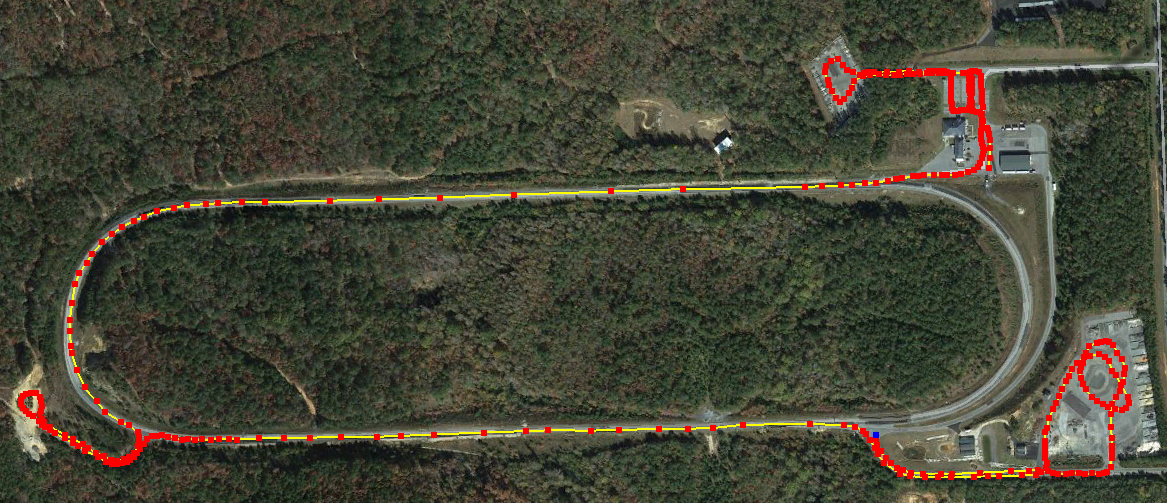
\includegraphics[width=5in]{./figs/varied_test_route.png}
%     \caption{Route taken for the varied driving test}
% \end{figure}


%%%%%%%%%%%%%%%%%
% Results section
\section{Results} \label{sec:results}

%%%%% Lane Change between Cones
\subsection{Lane Change Replication Test Results} \label{sec:lanechangetestresults}

\begin{figure}[ht] \caption{Results from all runs of the lane change replication test} \centering \label{fig:lanechangeresults}
    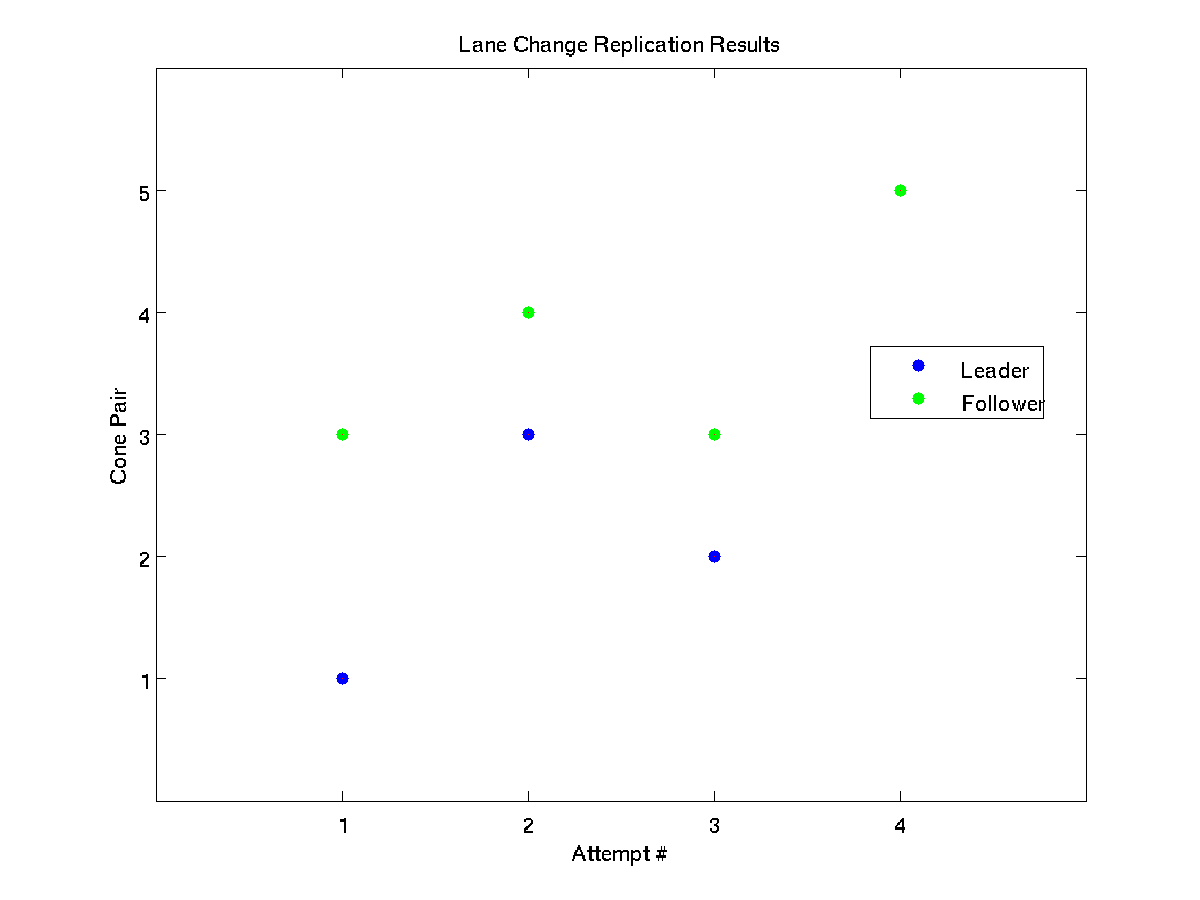
\includegraphics[width=4in]{./figs/lane_change_results.png}
\end{figure}

Figure \ref{fig:lanechangeresults} shows the results of all runs of the lane change replication test.

It is plain to see that in every instance where a lane change was made between the improper cone pair, the follower changed lanes later than did the leader. This is attributed to latency existing in the combined system from calculation and driver reaction.


%%%%% Follow the Path around the track
\subsection{Precision Following Test Results} \label{sec:precisionfollowingresults}

\begin{figure}[ht] \centering \label{fig:precisionresults_earth}
    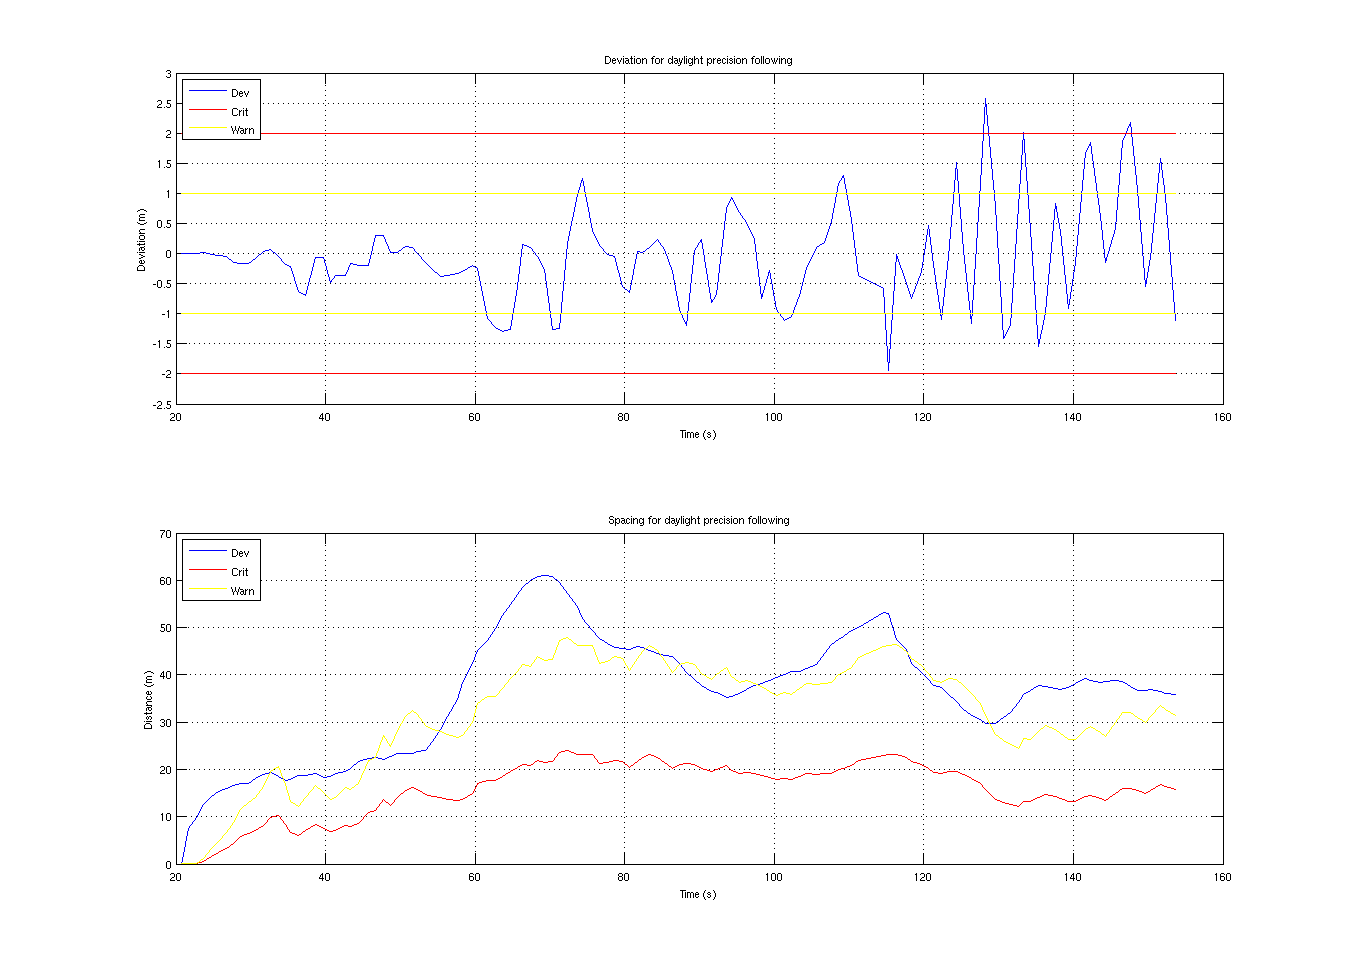
\includegraphics[width=5in]{./figs/dst_dev_earth_tracklap.png}
    \caption{Best run of the precision following test using Earth GUI}
\end{figure}

\begin{figure}[ht] \centering \label{fig:precisionresults_monolith}
    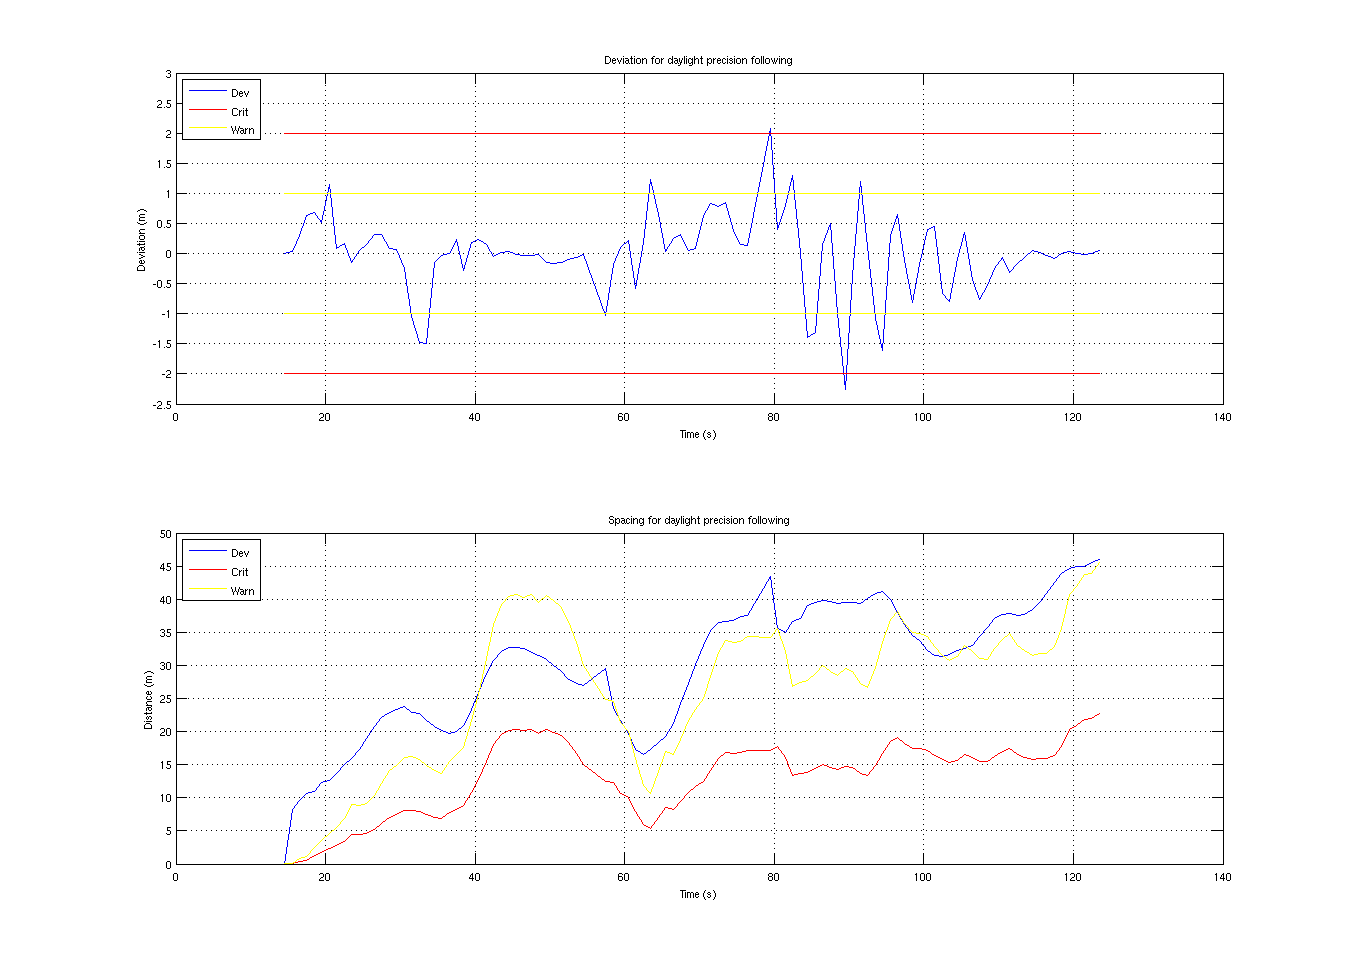
\includegraphics[width=5in]{./figs/dst_dev_monolith_tracklap.png}
    \caption{Best run of the precision following test using monolith GUI}
\end{figure}

Shown in Figs. \ref{fig:precisionresults_earth} \ref{fig:precisionresults_monolith} are the best of all runs of the precision following test. 

When at any point a path is uncalculable, due to satellite outage, outlying values, course errors, or other errors, the path reported is of length one (a single point at the position of the leader). When this occurs, the following distance becomes 0.0, and these instances are ignored in tabulation of the following distance score.

